\documentclass{report}
\usepackage{listings}
\usepackage[margin=1.0in]{geometry}
\usepackage{graphicx}
\usepackage{hyperref}
\usepackage{amsmath}
\hypersetup{colorlinks=true}
\usepackage[document]{}
\title{EECE.5200 - Homework 2}
\author{Travis Kessler}
\date{2 March 2021}
\begin{document}
	\maketitle
	\newpage

	% \lstset{language=shell}
	\lstset{frame=lines}

	\section*{Accessing Source Code}
	
	Source code is available at: \href{https://github.com/tjkessler/eece5200/tree/main/hw2}{https://github.com/tjkessler/eece5200/tree/main/hw2}
	
	\textit{}
	
	\noindent To compile the source code, navigate to the \textit{hw2} directory, and run "make". Each question's executable, "q1.o" and "q3.o", can then be executed from the terminal.
	
	\section*{Question 1}
	
	This question involves evaluating \textit{$A^{-1}B$} given:
	
	\textit{}
	
	$A = \begin{bmatrix}
		-2 & 1 & 2 \\
		2 & 3 & -2 \\
		1 & -2 & 3
	\end{bmatrix}$
	$B = \begin{bmatrix}
		-2 & 2 & 4 \\
		3 & 1 & -1 \\
		5 & -4 & 6
	\end{bmatrix}$

	\textit{}
	\textit{}
	
	\noindent Using GESS in the supplied port3 library, executing \textit{question\_1.f} (compiled as \textit{q1.o}), the following output was obtained:
	
	\begin{lstlisting}
		(base) tjkessler@Traviss-MacBook-Air hw2 % ./q1.o 
		  cond=   3.38068199    
		      0.22188E+01   -0.10938E+01
		      0.25000E+00    0.75000E+00
		      0.10938E+01   -0.46875E+00
	\end{lstlisting}

	\section*{Question 2}
	
	Given the three port resistor network such that the third port is open-circuit:
	
	\textit{}
	
	$V_{1} = R_{11}I_{1} + R_{12}I_{2}$
	
	$V_{2} = R_{12}I_{1} + R_{22}I_{2}$
	
	$V_{3} = R_{31}I_{1} + R_{32}I_{2}$
	
	\textit{}
	
	\noindent and:
	
	\textit{}
	
	$V = (1, 2, 3)^{T}$, $I = (1, 2)^{T}$
	
	\textit{}
	
	\noindent it is apparent that a system of three equations with 5 unknowns is present. The system can be written as:
	
	\textit{}
	
	$\begin{bmatrix}
		1 & 2 & 0 & 0 & 0 & \vdots & 1 \\
		0 & 1 & 2 & 0 & 0 & \vdots & 2 \\
		0 & 0 & 0 & 1 & 2 & \vdots & 3
	\end{bmatrix}$

	\textit{}
	
	\noindent or as the system:
	
	\textit{}
	
	$R_{11} + 2R_{12} = 1$
	
	$R_{12} + 2R_{22} = 2$
	
	$R_{31} + 2R_{32} = 3$
	
	\textit{}
	
	\noindent solving for $R_{12}$, the only common variable between multiple equations, we can simplify to:
	
	\textit{}
	
	$R_{11} - 4R_{21} = -3$
	
	$R_{31} + 2R_{32} = 3$
	
	\textit{}
	
	\noindent then, solving for the minimum values, we observe all resistances are equal to \textbf{1}. Therefore, solving for $R_{12}$ using known resistances, the resulting matrix of resistances is:
	
	\textit{}
	
	$R = \begin{bmatrix}
		1 & 0 \\
		0 & 1 \\
		1 & 1
	\end{bmatrix}$

	\section*{Question 3}
	
	\begin{figure}[!ht]
		\centering
		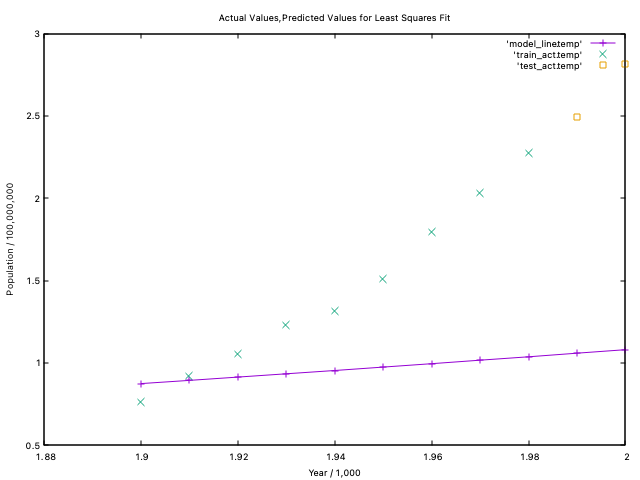
\includegraphics[scale=0.7]{figures/q3_results.png}
		\caption{Actual data versus least-squares line}
	\end{figure}

	Figure 1 compares the actual data, both for least-squares fitting and the two points used to test the model, to the predicted values generated from the least squares model (purple). While the inflection of the model with respect to the training data is correct (positive), the magnitude of the slope indicates an incorrect fit. This can likely be attributed to an incorrect implementation of the least-squares algorithm, and warrants further troubleshooting. It was found that the training set mean absolute error was \textbf{0.5026}, and the mean absolute error for the test set (two highest points) was \textbf{1.5851}.

	\begin{thebibliography}{99\kern\bibindent}
	
	\bibitem{hwref}
	Thompson, C.
	\textit{University of Massachusetts Lowell Department of Electrical and Computer Engineering 16.520 Computer Aided Engineering Analysis Problem Set 2}.
	Retrieved March 2, 2021, from http://morse.uml.edu/Activities.d/16.520/S2021.d/HW2.pdf
	
	\end{thebibliography}

\end{document}